\documentclass{beamer}
\mode<presentation>
\usepackage[utf8]{inputenc}
\usepackage{graphicx}
\usepackage[english,italian]{babel} % se non fosse inglese dovrei indicare la lingua nella quale sillabare [Italian]
%\usepackage{fancybox}
\useoutertheme{}
\usepackage{beamerthemeshadow}
\usepackage{ulem}
\usepackage{courier}
\usepackage{tikz}
\usepackage{listings}
\usepackage{amsfonts}
\usepackage{fontawesome5}
\usepackage{color,soul}
\usetikzlibrary{snakes}
%\usepackage{beamertexpower}
%\beamertemplatetransparentcovereddynamicmedium
\usetheme{GTER} %(se vuoi mettere l'autore)
\useinnertheme{rectangles}
%\useoutertheme{infolines}
\usecolortheme[RGB={151,215,0}]{structure}
%\usecolortheme[RGB={0,99,29}]{palette quaternary}

\setbeamercovered{transparent}
\setbeamerfont{frametitle}{size=\small,series=\bfseries}
\setbeamercolor{frametitle}{bg=gter!}

\definecolor{lightred}{rgb}{0.94,0.04,0.04}
\definecolor{aqua}{rgb}{0.00,0.80,1.00}
\definecolor{lightgreen}{rgb}{0.01,0.40,0.03}
\definecolor{limegreen}{rgb}{0.61,1.00,0.10}
\definecolor{peach}{rgb}{1.01,0.85,0.72}
\definecolor{purple}{rgb}{0.93,0.51,0.93}
\definecolor{indianyellow}{rgb}{0.98,0.75,0.30}
\definecolor{brick}{rgb}{0.70,0.13,0.13}
\definecolor{springsteen}{rgb}{0.00,0.49,0.19}
%%%%%%%%%%%%%%%%%%%%%%%%%%%%%%%%%%%%%%%%%%%%%%%%%%%%%%%%%%%%%%%%%%%%%%
% \definecolor{gter}{rgb}{0.00,0.49,0.22} %verde GTER estratto da gimp
\definecolor{gter}{RGB}{151,215,0}
%%%%%%%%%%%%%%%%%%%%%%%%%%%%%%%%%%%%%%%%%%%%%%%%%%%%%%%%%%%%%%%%%%%%%%
\definecolor{lightorange}{rgb}{1.01,0.50,0.00}
\definecolor{royalblue}{rgb}{0.25,0.41,1.00}
\definecolor{lightgray}{rgb}{0.94,0.94,0.94}

% \definecolor{links}{HTML}{2A1B81}
\hypersetup{colorlinks,linkcolor=lightgray,urlcolor=springsteen}

\usepackage{minted}

\title{Python 1}
\subtitle{Sintassi base}
\author[]{Gter srl Innovazione in Geomatica Gnss e Gis}
\author[]{Relatore: Simone Parmeggiani}

\logo{
\includegraphics[height=0.5 cm]{./Gter.png}}

\begin{document}
	{
		{
			\setbeamertemplate{footline}{} 
			\begin{frame}
				\titlepage
        \end{frame}
		}
		\addtocounter{framenumber}{-1}

\section{Introduzione}
\subsection{Introduzione}

\begin{frame}
   \frametitle{Cos'è Python}

   Python è un linguaggio di programmazione orientato agli oggetti noto per la sua chiarezza, potenza e flessibilità. Si tratta di un linguaggio interpretato, il che significa che un interprete legge ed esegue il codice direttamente, senza compilazione.


    \begin{figure}
        \centering
        
\includegraphics[width=0.3\linewidth]{pics/pylogo.png}
    \end{figure}

\end{frame}

\begin{frame}
   \frametitle{Cos'è Python #2}

    Creato da Guido van Rossum nel 1989 e rilasciato nel 1991, Python deve il proprio nome al gruppo comico Monty Python, di cui lo sviluppatore era un grande fan. Si tratta di un linguaggio rapido da apprendere, comprendere e usare, con una sintassi pulita e uniforme. La filosofia alla base della creazione di Python infatti si concentra principalmente sulla leggibilità e manutenibilità del codice.
    
    Il linguaggio viene fornito con una vasta libreria standard per l'elaborazione di stringhe, protocolli Internet, unit testing, registrazione, profilazione e analisi del codice Python, e interfacce del sistema operativo. Inoltre è possibile potenziare ed allargare le funzionalità di Python grazie alle estensioni di terze parti.
    
\end{frame}

\begin{frame}

   \frametitle{Perchè scegliere Python?}

    
    \begin{itemize}
        \item \textbf{Semplicità e velocità:} questo linguaggio semplifica notevolmente la programmazione.
        \item \textbf{Eleganza e flessibilità:} questo linguaggio offre molte possibilità al programmatore grazie alla sua facile leggibilità e interpretabilità.
        \item \textbf{Programmazione produttiva:} è semplice da imparare, con una curva di apprendimento moderata. È molto facile iniziare a programmare e promuove la produttività.
        \item \textbf{Ordine e pulizia:} è molto leggibile e i suoi moduli sono ben organizzati.
        \item \textbf{Portatilità:} è un linguaggio portatile. Oggi si può utilizzare Python praticamente con qualsiasi sistema.
        \item \textbf{Community:} ha un gran numero di utenti e tale comunità partecipa attivamente allo sviluppo del linguaggio.
    \end{itemize}

\end{frame}

\begin{frame}

   \frametitle{Limiti di Python}

    \begin{itemize}
        \item \textbf{Prestazioni:} come tutti i linguaggi di alto livello, non è possibile raggiungere profondità di operazioni.
        \item \textbf{Web:} Nonostante stiano uscendo librerie che aiutano, la programmazione web è difficile e macchinosa con python, meglio scegliere altri linguaggi.
        \item \textbf{Mobile:} allo stesso modo non è indicato per applicazioni mobile (anche se Ionic, Django, IronPython, Kivy stanno facendo progressi)
        \item \textbf{Gestione della memoria:} Python utilizza la gestione automatica della memoria (garbage collection), che può introdurre overhead e influire sulle prestazioni in alcuni scenari.
        \item \textbf{Multithreading}: Il Global Interpreter Lock (GIL) impedisce l'esecuzione di più thread Python, limitando l'efficacia del multithreading.
    \end{itemize}

\end{frame}

\section{Setup di Python}

\begin{frame}
    \frametitle{Installazione di Python}

    \href{https://www.freecodecamp.org/italian/news/come-installare-python-su-windows/}{Installazione in ambiente Windows}

    Aprire prompt dei comandi:
    python --version

\end{frame}


\begin{frame}

    \frametitle{Installazione IDE}

    \href{https://code.visualstudio.com/download}{Installazione VS Code in ambiente Windows}

    Un IDE, acronimo di Integrated Development Environment (Ambiente di Sviluppo Integrato), è un software applicativo che fornisce strumenti completi per lo sviluppo di software. Gli IDE sono progettati per facilitare la scrittura, il test e il debugging del codice sorgente. Ecco alcune delle principali caratteristiche e componenti di un IDE:

    \begin{itemize}
        \item \textbf{Editor di Codice:} Un editor di testo avanzato che supporta la sintassi di vari linguaggi di programmazione, con funzionalità come l'evidenziazione della sintassi, il completamento del codice e il refactoring.
        \item \textbf{Debugger:} Uno strumento per eseguire il codice in modalità di debug, consentendo di impostare breakpoints, ispezionare variabili, eseguire il codice passo dopo passo e identificare e correggere gli errori.
    \end{itemize}
    
\end{frame}

\begin{frame}

    \frametitle{Installazione IDE}

    Alcuni esempi popolari di IDE includono:

    \begin{itemize}
        \item \textbf{Visual Studio:} Un IDE completo sviluppato da Microsoft, molto usato per lo sviluppo di software su piattaforma Windows. e il refactoring.
        \item \textbf{PyCharm:} Un IDE specifico per lo sviluppo in Python, sviluppato da JetBrains.
    \end{itemize}
    
\end{frame}


\section{I costrtutti base di Python}

\begin{frame}
    
    \frametitle{Stampa a terminale:}

    \begin{itemize}
        \item  \mintinline{python}{print("Hello World!")}
    
        \item \mintinline{python}{print("multiple output with number", 1)}
    
        \item \mintinline{python}{print("First line", end='')}
                \mintinline{python}{print(" second line")}
    \end{itemize}


\end{frame}

\begin{frame}
    
    \frametitle{Variabili}
    In python non serve dichiarare le variabili.
    Ogni volta che si assegna un valore, viene automaticamente creata una variabile del tipo adeguato:

    \begin{itemize}
        \item  \mintinline{python}{number = 3}
    
        \item \mintinline{python}{decimal = 7.5}
    
        \item \mintinline{python}{stringa = "Hello World!"}
    \end{itemize}

    Provare:
    \mintinline{python}{print(type(number).__name__, number}

    Notale che l'int() in Python è infinito (non esiste int8, int32 ecc)

\end{frame}

\begin{frame}
    
    \frametitle{Riutilizzo delle Variabili}
    Se ad un'etichetta viene riassegnato un valore, il tipo può cambiare:

    \begin{itemize}
        \item  \mintinline{python}{number = 3}
    
        \item \mintinline{python}{number = "ciao"}
        
    \end{itemize}

    \mintinline{python}{print(type(number).__name__, number}

\end{frame}

\begin{frame}
    
    \frametitle{Principi di OOP}
    In python tutto è un oggetto, questo significa che ogni entità nel linguaggio, sia essa una variabile, una funzione, una classe, un modulo, un numero, una stringa, ecc., è un'istanza di una classe e quindi un oggetto. Questo principio è alla base del design orientato agli oggetti di Python (Object Oriented Programming).

    \begin{figure}
        \centering
        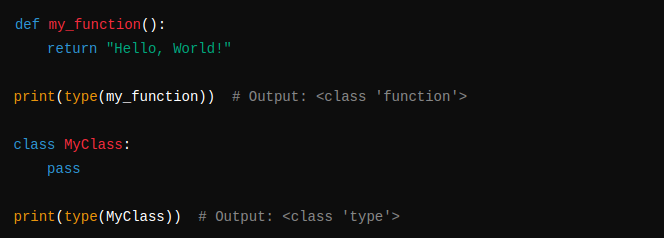
\includegraphics[width=1\linewidth]{pics/oop.png}
    \end{figure}


\end{frame}

\begin{frame}
    
    \frametitle{Principi di OOP 2}

    Vediamo un esempio con gli interi:
    
    \begin{itemize}
        \item \mintinline{python}{a = int('10')}
   
        \item \mintinline{python}{a = int('65000)}
        
    \end{itemize}

    \mintinline{python}{print(a.bit_lenght())}
    
\end{frame}

\begin{frame}
    
    \frametitle{Principi di OOP 3}

    Vediamo un esempio con le string:
    
    \begin{itemize}
        \item \mintinline{python}{b = "Hello World!"}
        \item \mintinline{python}{print(b.count('o'))}
        \item \mintinline{python}{print(b.upper())}
        \item \mintinline{python}{print(b.split()}
    \end{itemize}
    
\end{frame}

\begin{frame}
    
    \frametitle{Aggiungiamo un pò di interattività}

    Definire input di variabili:
    
    \begin{itemize}
        \item \mintinline{python}{name = input("Ciao! come ti chiami? ")}
        \item \mintinline{python}{print("Ciao fai esempio coi percento")}
        \item \mintinline{python}{print("Ciao {}").format(name)}
        \item \mintinline{python}{print(f"Ciao {name}, Benvenuto su Python!")}
     \end{itemize}
    
\end{frame}

\begin{frame}
    
    \frametitle{Assegnamenti multipli}
  
    \begin{itemize}
        \item \mintinline{python}{age, name = 41, "Simone}
        \item \mintinline{python}{print(f"{name} ha {age} anni")}
     \end{itemize}

     questo è molto utile per invertire due variabili:

    \begin{itemize}
        \item \mintinline{python}{age, name = name, age}
     \end{itemize}
    
\end{frame}

\begin{frame}
    
    \frametitle{Note sulle virgolette}
  
    \begin{itemize}
        \item ' ... ', '' ... '', ''' ... '''
        \item " ... ", "" ... "", """ ... """
    \end{itemize}

Gestire i caratteri speciali in questo modo è più semplice:

    \begin{itemize}
        \item \mintinline{python}{print('testo con l'apostrofo')}
        \item \mintinline{python}{print('testo con l\'apostrofo'}
    \end{itemize}

\end{frame}

\begin{frame}
    
    \frametitle{Altri costrutti base:}

    \begin{itemize}
        \item \textbf{Liste:} \mintinline{python}{lst = [1, 2, 3]}
        \item \textbf{Tuple:} \mintinline{python}{tpl = (1, 2, 3)}
        \item \textbf{Dizionari:} \mintinline{python}{dct = {'mela':1, 'pera': 5}}
    \end{itemize}

    Esistono anche i \textbf{set()} che sono liste contenenti valori \textbf{univoci}

\end{frame}


\begin{frame}
    
    \frametitle{Liste}
    definiamo una lista
    \mintinline{python}{lst = [1, 2, 3, 7, 10]}
    e vediamo alcuni metodi utili:
    \begin{itemize}
        \item \textbf{Indexing:} \mintinline{python}{print(lst[0])}
        \item \mintinline{python}{lst.append(5)}
        \item \mintinline{python}{lst.pop()}
    \end{itemize}

    L'indexing può essere eseguito anche sulle stringhe, che di fatto possono essere considerate liste di tanti caratteri concatenati.
    Questo permette anche operazioni di \textbf{slicing}

\end{frame}

\begin{frame}
    
    \frametitle{Tuple}
    definiamo una tupla
    \mintinline{python}{tpl = (1, 2, 3, 7, 10)}
    e vediamo gli stessi metodi:
    \begin{itemize}
        \item \textbf{Indexing:} \mintinline{python}{print(tpl[0])}
        \item \mintinline{python}{tpl[1] = 77}
    \end{itemize}

    La tupla è \textbf{immodificabile}, pertanto questa operazione ritornerà un errore.
    Si tenga presente che sia le tuple che le liste sono oggetti \textbf{ORDINATI}, vedremo che questo non è vero per i dizionari

\end{frame}

\begin{frame}
    
    \frametitle{Dizionari}
    definiamo un dizionario:
    \mintinline{python}{voti = {'simone': 7, 'maria': 8, 'luca': 5}}
    
    \begin{itemize}
        \item \textbf{Indexing:} \mintinline{python}{print(voti['simone'])}
        \item \mintinline{python}{voti['silvia'] = 7.5}
    \end{itemize}

    I dizionari \textbf{NON SONO ORDINATI} pertanto non potete fare affidamento all'ordine con cui vengono stampati (anche se a volte le chiavi vengono sempre stampate nello stesso ordine)

\end{frame}

\begin{frame}
    
    \frametitle{Set}

    \mintinline{python}{primo = {'simone', 'maria', 'luca'}}
    \mintinline{python}{secondo = {'silvia', 'andrea', 'maria'}}
    
    \begin{itemize}
        \item Unione: \mintinline{python}{print(primo | secondo)}
        \item Intersezione: \mintinline{python}{print(primo & secondo)}
        \item Differenza \mintline{python}{print(primo - secondo}
    \end{itemize}

\end{frame}

\begin{frame}
    
    \frametitle{Oggetti multipli}
    finora abbiamo definito gli oggetti per sè, ma niente impedisce di unirli tra loro creando liste di liste (comoda per oggetti bidimensionali) oppure salvare una lista come valore di un dizionario e così via aumentando la complessità potenzialmente all'infinito.
    
    Inoltre è possibile compilare questi oggetti con forme contratte chiamate \textbf{list comprehension e dict comprehension}

\end{frame}

\section{Controlli di flusso}

\begin{frame}
\begin{figure}

    \textbf{ATTENZIONE A NON INCROCIARE I FLUSSI ! ! !}
    \centering
    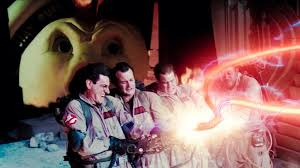
\includegraphics[width=0.75\linewidth]{flussi.png}
\end{figure}
\end{frame}

\begin{frame}
    \frametitle{Booleani e NULL value}
    \centering
     \mintinline{python}{True, False, None}
\end{frame}

\begin{frame}
    
    \frametitle{if - elif - else}
    \begin{figure}
        \centering
        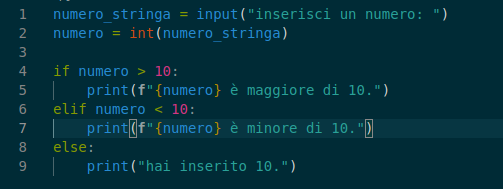
\includegraphics[width=1\linewidth]{if-elif-else.png}
    \end{figure}

\end{frame}

\begin{frame}
    
    \frametitle{for}
    \begin{figure}
        \centering
        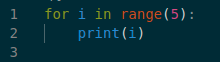
\includegraphics[width=1\linewidth]{for.png}
    \end{figure}

\end{frame}

\begin{frame}
    
    \frametitle{while}
    \begin{figure}
        \centering
        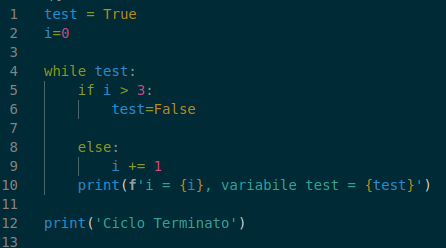
\includegraphics[width=1\linewidth]{while.png}
    \end{figure}

\end{frame}


\section{Funzioni}
\begin{frame}
    
    \frametitle{Funzioni}
    \begin{figure}
        \centering
        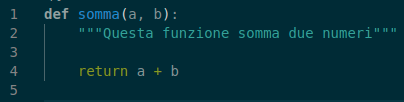
\includegraphics[width=1\linewidth]{funzioni.png}
    \end{figure}

    \textbf{Attenzione!} Non necessariamente le funzioni devono ritornare un risultato

\end{frame}

\begin{frame}
    
    \frametitle{Funzioni 2}

    \textbf{Attenzione!}
    \begin{itemize}
        \item \mintinline{python}{a = 1}
        \item \mintinline{python}{print(id(a))}
        \item \mintinline{python}{b = a}
        \item \mintinline{python}{print(id(b))}
        \item \mintinline{python}{print(a is b)}
    \end{itemize}
    
    A e B puntano allo stesso valore!
    se cambio il valore di a, es \mintinline{python}{a = 2}
    avrò un id diverso e a is b = False
    ma se rivalorizzo a = 1... ?

\end{frame}

\begin{frame}
    
    \frametitle{Funzioni 3}

    Le funzioni possono accettare parametri in ingresso, alcuni dei quali possono essere definiti di default mentre altri possono essere opzionali

\end{frame}

\section{Classi}

\begin{frame}

    \frametitle{Classi 1}
    \begin{figure}
        \centering
        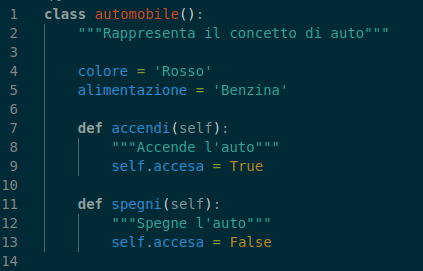
\includegraphics[width=1\linewidth]{image.png}
    \end{figure}

\end{frame}

\begin{frame}

    \frametitle{Classi 2}
        \begin{itemize}
        \item \mintinline{python}{ferrari = Automobile()}
        \item \mintinline{python}{print(macchina.colore)}
        \item \mintinline{python}{print(macchina.alimentazione)}
        \item \mintinline{python}{print(macchina.accesa)}
    \end{itemize}

    Errore perchè non esiste un attributo "accesa" di questa classe!
    "colore" e "alimentazione" sono \textbf{attributi statici} della classe, mentre "accesa" viene creata dai metodi della classe nel caso vengano eseguiti.
    Nel nostro esempio non abbiamo invocato nessun metodo quindi "accesa" non esiste ancora!
\end{frame}

\begin{frame}

    \frametitle{Classi 3}
        \begin{itemize}
        \item \mintinline{python}{ferrari = Automobile()}
        \item \mintinline{python}{lamborghini = Automobile()}
        \item \mintinline{python}{print(ferrari.colore, lamborghini.colore)}
        \item \mintinline{python}{automobile.colore='Bianco')}
        \item \mintinline{python}{ferrari.colore='Verde')}
        \item \mintinline{python}{print(ferrari.colore, lamborghini.colore))}
    \end{itemize}

    Errore perchè non esiste un attributo "accesa" di questa classe!
    "colore" e "alimentazione" sono \textbf{attributi statici} della classe, mentre "accesa" viene creata dai metodi della classe nel caso vengano eseguiti.
    Nel nostro esempio non abbiamo invocato nessun metodo quindi "accesa" non esiste ancora!
\end{frame}

\begin{frame}
    \frametitle{Costruttore}
    \begin{figure}
        \centering
        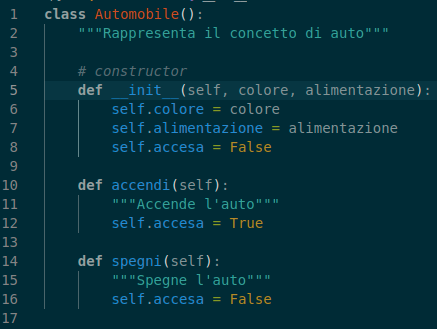
\includegraphics[width=0.75\linewidth]{constructor.png}
    \end{figure}
\end{frame}

\begin{frame}

    \frametitle{Costruttore 2}
        \begin{itemize}
        \item \mintinline{python}{ferrari = Automobile('rossa', 'GPL')}
        \item \mintinline{python}{print(ferrari.colore)}
        \item \mintinline{python}{print(ferrari.alimentazione)}
        \item \mintinline{python}{print(ferrari.accesa)}
        \item \mintinline{python}{ferrari.accendi()}
        \item \mintinline{python}{print(ferrari.accesa)}
    \end{itemize}

    In questo modo non corro il rischio di intervenire su variabili prima che vengano inizializzate.
    Esistono classi che gestiscono dinamicamente i propri metodi al fine di generare al volo oggetti (cosa che in altri linguaggi è difficilissimo!). Questa funzione è molto potente ma allo stesso tempo richiede molto metodo.

\end{frame}

\section{Link Utili}

\begin{frame}

    \frametitle{Link Utili}
    
    \href{https://www.codewars.com/}{https://www.codewars.com/}

    \href{https://www.hackerrank.com}{https://www.hackerrank.com}

    \href{https://codingbat.com/python}{https://codingbat.com/python}

    \href{https://coding-gym.org/}{https://coding-gym.org/}
    
\end{frame}


\section{Contatti e licenze}
\subsection{Contatti e licenze}
{
\setbeamertemplate{footline}{} 
\setbeamertemplate{headine}{} 
\frame{	
\addtocounter{framenumber}{-1}  % non conto questa slide
\begin{center}
\bigskip

\includegraphics[width=0.2\textwidth]{./Gter.png} \\ 
\scriptsize{
%Gter srl Innovazione in Geomatica Gnss e Gis\\

Via Jacopo Ruffini 9/1A\\
16128, Genova \\
formazione@gter.it\\}
\normalsize
\bigskip
\href{www.gter.it}{\textcolor{gter}{\emph{www.gter.it}}}
	
\bigskip	

  	\href{https://twitter.com/@gteronline} { 
\includegraphics[width=0.15\textwidth]{./tw.jpg}}
	\hspace{30pt}
	 \href{http://www.facebook.com/Gteronline} { 
\includegraphics[width=0.15\textwidth]{./fb.jpg}}
		\hspace{30pt}
%	 \href{ https://plus.google.com/+GterIt/posts} { \includegraphics[width=0.15\textwidth]{../go.png}}
%	 \hspace{30pt}
	 \href{http://www.linkedin.com/company/gter-srl-innovazione-in-geomatica-gnss-e-gis} { 
\includegraphics[width=0.15\textwidth]{./ln.png}}
	 
	 
	 

	 
\bigskip
\vspace{30pt}

	
	\href{http://creativecommons.org/licenses/by-sa/3.0/deed.it} {	
	
\includegraphics[width=0.15\textwidth]{./88x31.png} 
	\\	
	\tiny Quest' opera è distribuita con licenza Creative Commons Attribuzione - Condividi allo stesso modo 3.0 Unported.} 	
	
	
	
\end{center}
%\tableofcontents[pausesections,part=2]
}
}

\end{document}
